\documentclass[11pt,a4paper]{article}
\usepackage{lmodern}
\usepackage[utf8]{inputenc}
\usepackage[T1]{fontenc}
\usepackage{amsmath,amssymb}
\usepackage{graphicx}
\usepackage{booktabs}
\usepackage[hidelinks]{hyperref}
\hypersetup{
  pdftitle={FIRE: Fisher Information Recommendation Engine},
  pdfauthor={Jung Min Kang},
  pdfsubject={Psychometric content routing for recommendation systems},
  pdfkeywords={recommender systems, item response theory, Fisher information, LLTM}
}
\usepackage{natbib}
\usepackage[margin=1in]{geometry}
\usepackage{algorithm}
\usepackage{algorithmic}
\usepackage{subcaption}
\usepackage{placeins}

\title{FIRE: Fisher Information Recommendation Engine\\[4pt]
\large Psychometric Content Routing for Recommendation Systems}

\author{Jung Min Kang\\
Independent Researcher, Seoul, South Korea\\
\texttt{gangjeongmin23@gmail.com}\\
ORCID: 0009-0007-9599-2792}

\date{May 2026}

\begin{document}
\maketitle

\begin{abstract}
We introduce FIRE (Fisher Information Recommendation Engine), a recommendation algorithm grounded in Item Response Theory (IRT) and the Linear Logistic Test Model (LLTM). FIRE operationalizes the PCR frontier value, $P(1-P)$, as a Fisher-information-shaped exploration term; for warm IRT-scored items this reduces to the standard local Fisher information criterion used in computerized adaptive testing. FIRE combines (1)~IRT-based engagement prediction for exploitation, (2)~normalized Fisher Information for exploration, and (3)~an LLTM item-feature-based difficulty prior for low-count items. On MovieLens-1M~\citep{harper2015movielens} (6,040 users, 3,883 valid movies), with full-catalog candidate evaluation over 300 randomly sampled eligible users per seed across 3 seeds, FIRE achieves AUC $0.7682 \pm 0.0002$ and provides 1.8$\times$ more catalog coverage than IRT among learned models ($0.0179$ vs $0.0100$), with explicit per-component score decompositions. LLTM achieves a squared correlation of $\rho^2 = 0.564$ between 22 observable item features and fitted warm-item difficulty, in-sample. On low-count items, LLTM interpolation did not improve prediction over IRT, indicating that FIRE's current empirical advantage is catalog coverage rather than cold-start accuracy. In the included implementation, the core model completes in approximately 97 seconds per seed in local CPU runs; runtime may vary with hardware and numerical-library threading.
\end{abstract}

\section{Introduction}

Social media recommendation systems share a multi-objective scoring structure. A leaked internal TikTok document describes a simplified value-weighted formula based on predicted interactions~\citep{tiktok_algo}; we use this as an architectural analogy only, not as an official platform specification. Similar scoring underlies YouTube's two-stage pipeline~\citep{covington2016youtube} and Meta's content systems~\citep{meta2023ai}.

FIRE is motivated by cold-start, diversity, and transparency challenges~\citep{kaminskas2016diversity,euaiact}, but in this MovieLens-1M experiment its demonstrated empirical advantage is catalog coverage among learned models, not cold-start accuracy. FIRE builds on psychometric theory: the Frontier Value $F = P(1-P)$ from PCR~\citep{kang2026pcr} is mathematically equivalent to Fisher Information~\citep{lord1968}---the criterion BanditCAT~\citep{sharpnack2024banditcat} uses for adaptive item selection. Recent work has applied multidimensional IRT directly to MovieLens-1M, showing that MIRT can support interpretable latent profiles and exploration--exploitation control~\citep{veldkamp2025mirt}.

\section{The FIRE Algorithm}

\begin{equation}
\text{FIRE}(u, i) = \alpha_u \cdot P_{\text{eff}}(u,i) + (1 - \alpha_u) \cdot \bar{I}(u,i)
\end{equation}

$P_{\text{eff}} = (1 - \lambda_i) \cdot \sigma(a_i(\theta_u - b_i)) + \lambda_i \cdot \sigma(-\mathbf{q}_i^\top \boldsymbol{\eta})$ interpolates IRT (warm items) and an LLTM item-feature-based difficulty prior~\citep{fischer1973} (low-count items).

$\bar{I} = a_i^2 \cdot P_{\text{eff}}(1 - P_{\text{eff}}) / I_{\max}$ is a normalized Fisher-information-shaped exploration term; for warm items where $\lambda_i = 0$, this reduces to standard 2PL Fisher information.

$\alpha_u = \sigma(\log(n_u / N_0))$ adapts from exploration to exploitation. $\lambda_i = \max(0, 1 - n_i / M_0)$ weights LLTM for low-count items.

\begin{algorithm}[H]
\caption{FIRE Recommendation}
\begin{algorithmic}[1]
\REQUIRE Training data, item features $\mathbf{Q}$, thresholds $N_0, M_0$
\STATE Fit IRT: $\{\theta_u, b_i, a_i\}$ via SGD
\STATE Fit LLTM on warm items ($n_i \geq M_0$): $\boldsymbol{\eta} = (\mathbf{Q}_w^\top\mathbf{Q}_w + \lambda\mathbf{I})^{-1}\mathbf{Q}_w^\top\mathbf{b}_w$
\FOR{user $u$, full candidate catalog $\mathcal{C}_u$}
    \STATE Score, rank, return top-$K$
\ENDFOR
\end{algorithmic}
\end{algorithm}

\section{Experimental Setup}

\textbf{Data.} MovieLens-1M~\citep{harper2015movielens}: 6,040 users, 3,883 valid movies (max ID 3,952; 69 missing IDs excluded), 1,000,209 ratings. Temporal 80/20 split per user. Binary: rating $\geq 4$.

\textbf{Features.} 22 features from training data only (no test leakage): 18 genres (indexed by movie ID), log-popularity, average rating, rating std, year.

\textbf{LLTM.} Fitted on warm items only ($n_i \geq 10$). The LLTM component provides an item-feature-based difficulty prior, not a user-conditioned prediction. Reported squared correlation is in-sample.

\textbf{Training.} All models (IRT, SVD, FIRE) are fitted via stochastic gradient descent. For computational consistency across baselines, each SGD epoch uses a random subsample of up to 100,000 training interactions.

\textbf{Baselines.} IRT 1D, SVD-50, Popularity (Positive-count MostPop: items ranked by training positive-interaction count; the same scoring is used for both AUC and Top-K evaluation).

\textbf{Evaluation.} Full-catalog candidates (no sampling): each model scores all valid unrated items per user. 300 randomly sampled eligible users per seed. Coverage denominator: all 3,883 valid items. All results: 3 seeds, mean $\pm$ SEM. Because only three seeds are used, SEM values are descriptive rather than formal uncertainty estimates.

\section{Results}

\begin{table}[h]
\centering
\caption{AUC on temporal held-out interactions (mean $\pm$ SEM, 3 seeds).}
\label{tab:auc}
\begin{tabular}{lcc}
\toprule
Method & AUC & $\Delta$ vs Pop \\
\midrule
SVD-50 & $\mathbf{0.7823 \pm 0.0000}$ & $+0.1015$ \\
IRT 1D & $0.7766 \pm 0.0002$ & $+0.0958$ \\
FIRE & $0.7682 \pm 0.0002$ & $+0.0874$ \\
Pop & $0.6808 \pm 0.0000$ & --- \\
\bottomrule
\end{tabular}
\end{table}

\begin{table}[h]
\centering
\caption{Top-10 recommendation, full-catalog evaluation (mean $\pm$ SEM, 3 seeds, 300 users/seed).}
\label{tab:topk}
\begin{tabular}{lcccc}
\toprule
Method & Recall@10 & NDCG@10 & HitRate@10 & Coverage \\
\midrule
Pop & $0.0560 \pm 0.0019$ & $0.1077 \pm 0.0058$ & $0.447 \pm 0.013$ & $0.0189 \pm 0.0011$ \\
SVD & $0.0227 \pm 0.0019$ & $0.0441 \pm 0.0022$ & $0.262 \pm 0.012$ & $0.0162 \pm 0.0008$ \\
IRT & $0.0230 \pm 0.0013$ & $0.0406 \pm 0.0012$ & $0.263 \pm 0.007$ & $0.0100 \pm 0.0004$ \\
FIRE & $0.0185 \pm 0.0007$ & $0.0346 \pm 0.0011$ & $0.230 \pm 0.003$ & $0.0179 \pm 0.0005$ \\
\bottomrule
\end{tabular}
\end{table}

Popularity dominates Top-K accuracy (HitRate 44.7\%) and absolute coverage (0.0189), consistent with Ji et al.~\citep{ji2020popularity}. Among the learned models, FIRE achieves the highest coverage (0.0179), 1.8$\times$ that of IRT (0.0100), while trading accuracy for diversity: HitRate 23.0\% vs IRT's 26.3\%.

\begin{figure}[h]
\centering
\begin{subfigure}[t]{0.48\textwidth}
    \centering
    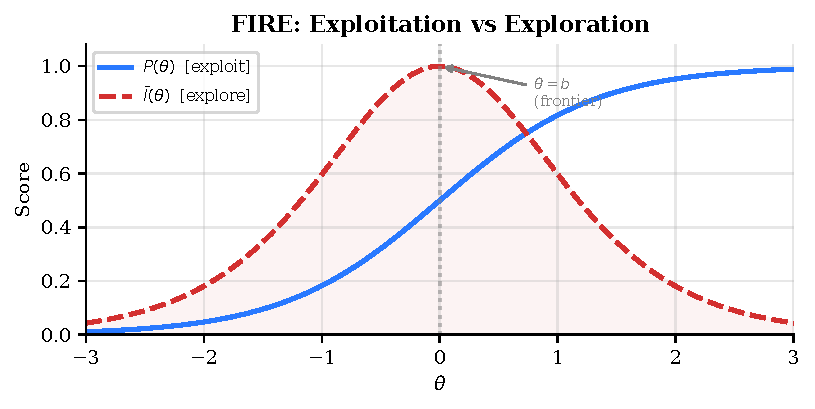
\includegraphics[width=\textwidth]{figures/fig1_concept.pdf}
    \caption{FIRE exploitation $P$ vs exploration $\bar{I}$. Fisher Information peaks at $\theta = b$.}
\end{subfigure}\hfill
\begin{subfigure}[t]{0.48\textwidth}
    \centering
    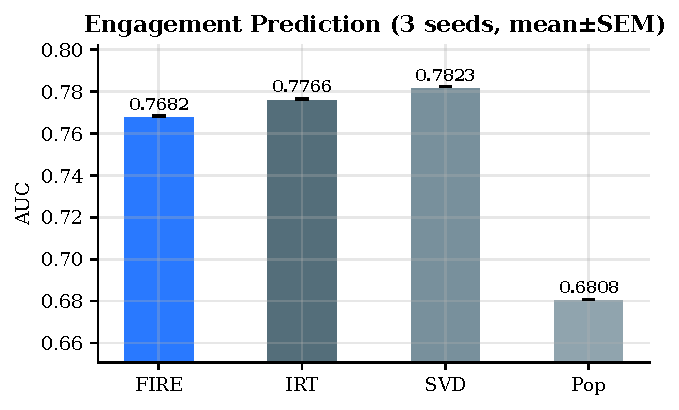
\includegraphics[width=\textwidth]{figures/fig2_auc.pdf}
    \caption{AUC (3 seeds). All learned models outperform MostPop.}
\end{subfigure}
\caption{FIRE mechanism and engagement prediction.}
\end{figure}

\begin{figure}[h]
\centering
\begin{subfigure}[t]{0.48\textwidth}
    \centering
    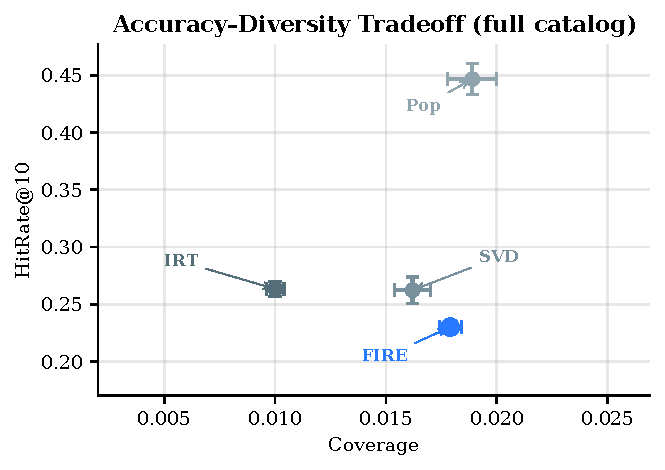
\includegraphics[width=\textwidth]{figures/fig3_tradeoff.pdf}
    \caption{Accuracy--diversity tradeoff. FIRE covers 1.8$\times$ more items than IRT among learned models.}
\end{subfigure}\hfill
\begin{subfigure}[t]{0.48\textwidth}
    \centering
    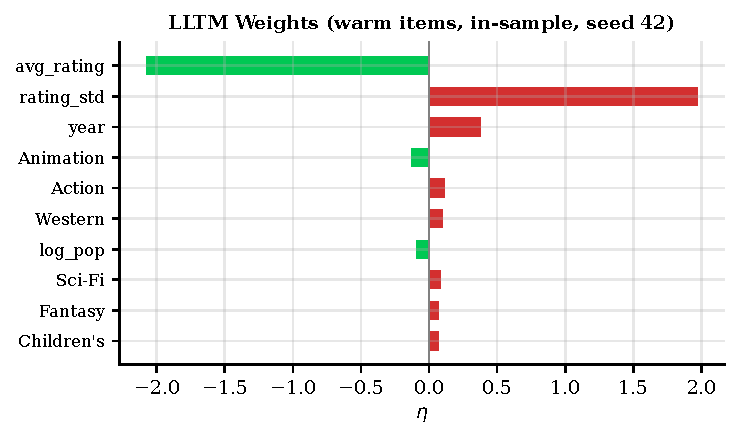
\includegraphics[width=\textwidth]{figures/fig4_lltm.pdf}
    \caption{LLTM weights (seed 42, warm items, in-sample). Average rating drives engagement ease.}
\end{subfigure}
\caption{Coverage tradeoff and LLTM feature decomposition.}
\end{figure}

\subsection{LLTM Feature Decomposition}

LLTM achieves an in-sample squared correlation of $\rho^2 = 0.5639 \pm 0.0023$ between 22 observable features and fitted warm-item IRT difficulty. Out-of-sample predictive validation remains future work.

\subsection{Low-Count Items}

On items with fewer than $M_0 = 10$ training interactions, IRT achieves AUC 0.6643, outperforming FIRE (0.6162) and Popularity (0.6012). The LLTM interpolation mechanism does not improve low-count item prediction on this dataset. True zero-shot new-item evaluation remains future work.

\subsection{Explainability}

FIRE provides explicit per-component score decompositions: $\theta_u$, $b_i$, $P_{\text{eff}}$, $\bar{I}$, $\alpha_u$, $\lambda_i$, and LLTM feature weights. Compared with many black-box ranking pipelines, FIRE exposes score components that can be inspected individually. This structure may support transparency-oriented documentation under frameworks such as the EU AI Act~\citep{euaiact}. This paper does not make a legal compliance claim.

\FloatBarrier
\section{Platform Mapping}

FIRE maps onto existing architectures as a complement, not a replacement: for TikTok-style interest-graph systems, it could add an adaptive Fisher-information signal alongside static business weights; for YouTube-style two-stage systems~\citep{covington2016youtube}, it can serve as an interpretable candidate pre-filter; and for Facebook-style discovery feeds, where AI-recommended content from unfollowed accounts constituted more than 20\% of feed content as of 2023~\citep{meta2023ai}, it can provide transparent routing for new content.

\section{Limitations}

(1)~SVD-50 outperforms FIRE on AUC. (2)~IRT outperforms FIRE on Recall, NDCG, and HitRate; FIRE's advantage is coverage among learned models. (3)~Low-count item prediction does not benefit from LLTM interpolation. (4)~LLTM squared correlation is in-sample. (5)~Popularity dominates Top-K accuracy and absolute coverage~\citep{ji2020popularity}. (6)~Single dataset; generalization is untested. (7)~SEM over 3 seeds is descriptive.

\section{Conclusion}

FIRE connects IRT, Fisher Information, and LLTM into a recommendation algorithm with adaptive exploration-exploitation. On MovieLens-1M with full-catalog evaluation, FIRE provides 1.8$\times$ more coverage than IRT among learned models, while retaining nontrivial accuracy and offering explicit per-component score decompositions.

\paragraph{Code.} Repository: \url{https://github.com/testofschool/fire-recommendation}.

\bibliographystyle{plainnat}
\bibliography{references}
\end{document}
